
Laeva ehitusel on vaja välja selgitada laeva parameetrid, mis vastaksid eelnevalt sätestatud tingimustele. Samuti märgitakse laeva parameetrid hiljem ka laeva käsiraamatusse. Nende parameetrite välja selgitamiseks on loodud käigukatsed, kus laev läbib määratud teekonna, mille käigus tehakse käsitsi mõõtmised, mida kasutatakse hiljem laeva võimekuse hindamiseks ja tulevaste ehitatavate laevade arendamiseks.

Laevade käigukatsed on vajalikud mõõdistuste täpsuse ja katsete reprodutseerimiseks. Lõputöö kirjutamise hetkel tehakse mõõdistusi küll täpsete seadmetega, kuid laevu juhivad erinevad inimesed ning tulemuste registreerimine käib manuaalselt, mis põhjustab ebatäpsusi ega taga katsete ühtset korratavust.

Käsitsi läbiviidavatel käigukatsetel esinevad mitmed probleemid:

\begin{enumerate}
\def\labelenumi{\arabic{enumi}.}
\item
  Mõõtetulemuste erinevused, mis sõltuvad laeva operaatori reaktsioonist ning psühholoogilisest seisundist
\item
  Kuna laeva juhib käigukatsetel üldjuhul üks isik, siis peab ta mitmete tegevuste jälgimisega paralleelselt tegelema, et andmeid koguda, see omakorda tähendab osalist andmekadu teatud perioodil
\item
  Mõõteandmete sisestamine ei ole automaatne, protokolli koostamine on mahukas ning nõuab mitme inimese koostööd
\item
  Laeval puudub arusaam teda ümbritsevast keskkonnast (võimekus iseseisvalt situatsioonides toime tulemisega ning õnnetuste vältimisega), seetõttu langeb ka see ülesanne laeva kaptenile, kes võib tähelepanematuse tõttu tekitada kriitilisi olukordi või põhjustada õnnetusi
\end{enumerate}

Seetõttu on mõistlik käigukatseid automatiseerida. Selleks oleks tarvis lisada laevale autonoomsust võimaldavad omadused, mis võimaldavad laeval katseid autonoomselt teha ning katsete käigus ka andmeid ise logida.

Autonoomne süsteem edastab laevale konkreetsed navigeerimiskäsklused ja salvestab andmed määratud perioodi jooksul. Kogutud materjali põhjal selguvad täpsed tulemused. Näiteks lainetes liikuva laeva kiirus on alati muutlik, mistõttu mõõdetud kiirus on otseses seoses registreerimise momendiga. Analüüsides valitud salvestusperioodi andmeid, on võimalik määrata laeva kiiruse karakteristikud katse toimumisel. Eelprogrammeeritud käigukatsed aitavad vältida juhtide erinevusi, näiteks laeva pööramise kiirus ning selleks kulunud aeg sõltub juhi intuitsioonist ja muudest isikuomadustest, mis omakorda takistavad laeva maksimaalse võimekuse objektiivset hindamist \cite{ref13} (vt Joonis~\ref{fig:image4}).

\begin{figure}[H]
\centering
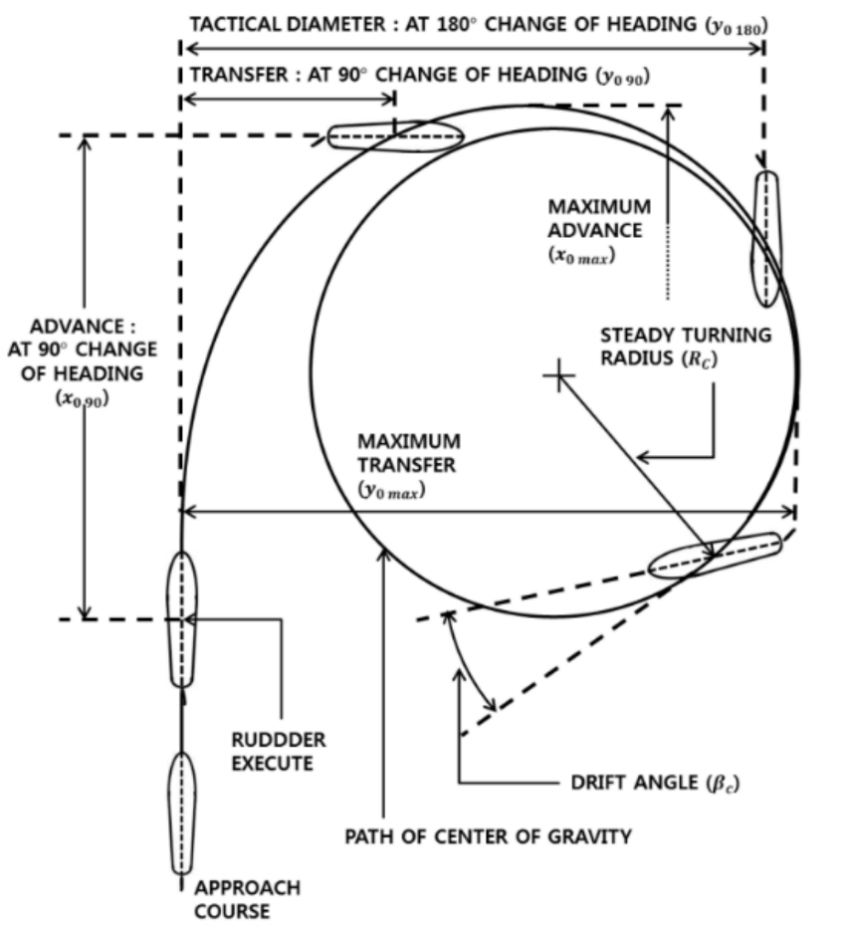
\includegraphics[width=4.70017in,height=5.14081in]{media/image4.png}
\caption{Laeva pöörderaadiuse mõõtmiseks loodud käigukatse \cite{ref13}}\label{fig:image4}
\end{figure}

Automaatsete käigukatsete jooksul kogutud info annab hea ülevaate laeva projekteerijatele ning inseneridele, mis omakorda on suureks abiks võimekamate laevade projekteerimisel ning olemasolevate veesõidukite arendamisel.
